\documentclass[a4paper,12pt]{article}

%%% Работа с русским языком
\usepackage{cmap}					% поиск в PDF
\usepackage{mathtext} 				% русские буквы в формулах
\usepackage[T2A]{fontenc}			% кодировка
\usepackage[utf8]{inputenc}			% кодировка исходного текста
\usepackage[english,russian]{babel}	% локализация и переносы

\usepackage{amsmath,amsfonts,amssymb,amsthm,mathtools} % AMS
%%% Работа с картинками
\usepackage{graphicx}  % Для вставки рисунков
\usepackage[overload]{empheq} % Для рамки в формулах

\begin{document}

\section{Теорема Лагранжа о среднем значении}

Теорема Лагранжа о среднем значении немного теоретическая, но она позволит нам познакомится с идеей интегрирования за пару лекций. Интегрирование будет изучаться на второй половине данного курса. Мы будем использовать аббревиатуру "TCЗ" при её обсуждении.

Говоря простым языком, "ТСЗ" говорит нам, что если пролетели 3000 км за 6 часов, то в какой момент полета вы будете лететь со скоростью 500 км/ч. (Потому что ваша средняя скорость и есть 500 км/ч)

Именно поэтому теорема и имеет название "теорема о среднем значении".

Говоря математическим языком:

\begin{empheq}[box=\fbox]{align*}
  \frac{f(b)-f(a)}{b-a}=f'(c) \text{ для некоторых $c$, $a<c<b$} \\
  \text{При условии, что $f$ дифференцируема на отрезке $a<x<b$, и непрерывна на  $a \leqslant x \leqslant b$}
\end{empheq}

\textbf{Геометрическое доказательство TCХ}: Представим график функции $f(x)$. Здесь,
$\frac{f(b)-f(a)}{b-a}$ является угловым коэффициентом секущеей линии через точки $(a, f (a))$ и $(b, f (b))$, и $f'(c)$ это угловой коэффициент касательной к графику функции. Нам нужно показать, что где-то между точками $a$ и $b$ есть точка на графике $(c, f (c))$, в которой угловые коэффициенты касательной и секущей равны.

\begin{figure}[ht]
\centering
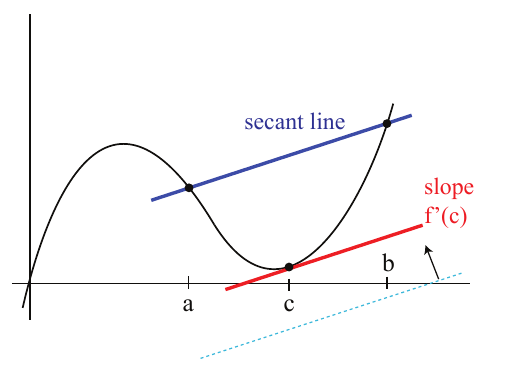
\includegraphics[height=6cm]{fig1.png}
\caption{Изображение теоремы о среднем}
\label{mvt}
\end{figure}

Проведя (заштрихованные) линии, параллельные секущей, на рисунке \ref{mvt} и будем двигать их вверх с низу графика, пока одна из них не коснется участка графика, лежащего между $a$ и $b$. Если же не коснется ни одна, то проведем штрихованную линию над графиком и будемт сдвигать их вниз до касания.

Читая доказательство, вы должны думать о том почему эта гипотеза необходима. Работало бы доказательство, если функция была разрывной или недифференцируемой?

Нам нужна гипотеза о непрерывности функции $f$, потому что если можете сидеть еще шесть часов, а затем телепортируетесь на 3000 км, то не будет момента времени, в котором ваша скорость была бы равна 500 км/ч. Теорема о среднем значении не дает гарантий относительно разрывных функций.

А что если функция не дифференцируема? Пусть $f(x)=|x|$. Тогда заштризованная линия будет всегда касаться графика в точке $x=0$, вне зависимости от секущей (смотри рисунок \ref{ruinmvt}). Даже если функция $f$ дифференцируема везде, кроме точки $x=0$, теорема о среднем неприменима здесь; нам нужно, чтобы $f'(x)$ существовала на $всех x$ между $a$ и $b$.

\begin{figure}[ht]
\centering
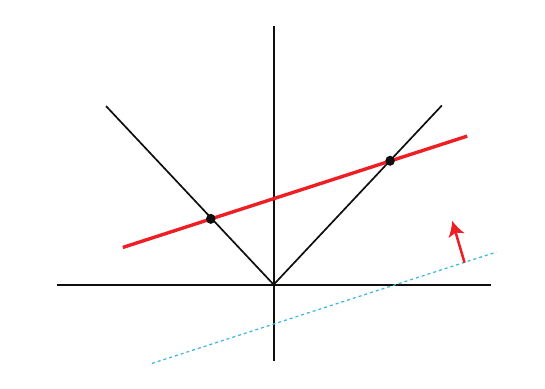
\includegraphics[height=6cm]{fig2.png}
\caption{График функции $y=|x|$ с секущей линией.(Одна плохая точка рушит все доказательство.)}
\label{ruinmvt}
\end{figure}

\textbf{Вопрос}: Что если линии, параллельные секущей, касаются графика в нескольких точках?

\textbf{Ответ}: Чем больше, тем лучше! График может изгибаться в нескольких местах и линия может касаться его хоть десять раз, или $f$ может быть константой и линия не коснется графика ни в одной точке. В математике, когда мы утверждаем, что одной точке верно, то это не обязательно значит, что это неверно для других

Тот факт, что эта точка существует как точка касания; мы можем увидеть, почему она должна существовать, однако мы на самом деле не доказали этого. Формальное доказательство связано с существованием касательных линий и использует другие приемы, чем те, которые мы изучаем в этом курсе.
\end{document}	